
\documentclass[11pt]{article}
\usepackage{graphicx}
\begin{document}


\title{Geometron: A Universal Language for Graphical Communication}
\author{Lafe Spietz}

\abstract{This is a white paper describing the basic construction of Geometron and how it can be of use specifically to the quantum information community.  Geometron is a metalanguage based on discrete geometric actions used to build symbols in a systematic way.  The basis of Geometron is the Geometron Virtual Machine(GVM), a purely geometric virtual machine in which points in space map to actions which have geometric meaning.  This paper first motivates the work by surveying existing languages used in the quantum information community, then describes the ideas behind the GVM and gives examples of how it is used in practical work.  A deep dive section into the exact structure and implementation of the GVM used here is then provided.  Finally the workflow is described which members of the QI community can immediately start to implement, and then future work is described which can leverage the power of geometry based thinking about quantum information for both better communication between the people in the community and better ways to program quantum computers more efficiently.}

\section{Motivation}

    Graphical communication is a fundamental component of building any new technology.  Often the more unfamiliar a technology is, the more we need to rely on simple cartoons and diagrams to tell others about it.  This communication between the people who create the new ideas and other people is fundamental, and can either make or break a new technology.   

    Our existing theoretical models for understanding new machines tend to ignore how machines propagate through the human population, but I believe this is a mistake.  These questions get banished from technical theoretical problems because we have arbitrarily divided who thinks about what problems up into ``engineering", ``humanities", ``marketing", etc.  We like to think that quantum computing will either succeed or fail based on some intrinsic technical merit, but none of us will ever succeed in this venture without clear communication between the advocates of the technology and the sponsors(funding agents, investors, upper managers).  Those people expect very simple and clear stories to be told in a mostly graphical format via PowerPoint, and that story must be more compelling than that of competing technologies.  Thus clear graphical communication is fundamental to the very survival of a new technology.  


    Graphical communication is also used to propagate our ideas outside of narrow sub-fields, expanding the number of minds focused on the problem.  What starts as a tiny minority of presenters at the American Physical Society March Meeting has taken over a huge fraction of all physics conferences, thanks in part to spreading the ideas of quantum information effectively in these venues.  This also depends on clear and simple graphics, as that is the only way to get a message across in a 10 minute talk.  


    As a technology transitions from the lab to the market place, graphical communication becomes even more critical, as creators of technology vie for a very limited attention span of potential users, almost entirely via web-based communication.  Quantum computing is now at a stage where it is attracting both user dollars and investor dollars, and a quick survey of leading commercial quantum computer ventures shows that very simple sequences of pictorial communication are becoming dominant.    

    Quantum Mechanics and quantum information science have always been particularly dependent on custom graphical languages.  Two examples that immediately come to mind are Feynman diagrams and the Bloch Sphere.  In both cases, ideas are expressed for which we also have words, numerical simulations and algebraic equations.  However in both cases, reducing all that to a simple cartoon totally changes how we are able to engage with problems, and makes a huge difference both in the ability to learn and do research in the respective problems they address.


    As quantum computing technology has become a part of the computer industry over the last few years, we have seen a number of efforts to build languages targeted specifically at programming quantum processors.  These languages are generally intended as part of a ``quantum stack'' which goes from the physical qubit layer up to the highest level where the end user will ultimately be solving their problem in quantum chemistry or number theory or whatever.  Rigetti Computing, IBM, Microsoft, and several other companies have all created such languages.  All of them are very clearly heavily influenced by the history of software written for classical information processors. The languages tend to look like C, Python, or Fortran, and to think about information the same way we all learned in classical computing, in terms of numbers and gates.  


    I would argue that all these approaches are limited by their divorce from the geometric nature of quatum information.  At the very least, adding a geometric layer to the quantum stack will allow for rapid, automated documentation to be created which makes the underlying code easier to interact with.  By having a language based on discrete symbols which correspond to gates, we can translate between that language, the actual physical gates, and the code in the various languages people have already written.  Thus at the very least, building the quantum Geometron language will allow for rapid, universal documentation to be created, making it easier for everyone using the various competing languages to rapidly communicate ideas online, and internally document their work.  


    This will be discussed in detail in another white paper, but part of the long term goal of this work on building geometric languages for quantum information is to create a fundamentally geometric way of interacting with the processors, without dealing directly with numbers at all.  Ideally, a problem we seek to solve can be posed geometrically, which is straightforward in instances such as protein folding or certain types of optimization. Then, using purely geometry-based languages similar to the one presented here, we build maps from the problem space to a Web browser and from the Web browser to the Hilbert space of the quantum information processor.  


    To understand why a new language for dealing with graphics in quantum information science is useful, it's worth examining the existing workflows used in the field for graphical communication.  We generally present our pitches for funding and support via PowerPoint slides, typically with simple graphics based on a lot of conceptual cartoons and diagrams.  Similarly we present to colleagues at conferences and colloquia in this format, but generally with greated detail in the technical diagrams.  We also communicate with investors, perspective customers(for for profit ventures) and with the general public using rapid communication over the Web, often via a marketing or PR department.  New types of diagram are generally created in vector format using Adobe Illustrator.  These graphics are then propagated through PowerPoint, web design software, and other parts of the Adobe suite before being used to communicate.  




\section{The Geometron Virtual Machine}

    The Geometron Virtual Machine is a function which maps discrete points in space to actions which manipulate discrete geometry.  That is the most general possible definition, which encompasses an infinite number of potential instances we might choose to create.  The GVM I'll be describing here is the Geometron Hypercube, which works in a Web Browser, and is written entirely in JavaScript.   


    Rather than trying to formalize the math of this idea, I will dive in and describe the specifics of the Geometron Hypercube used in all the work documented here.  This consists of two cubes, each with 8x8x8 = 512 cells.  Each cell has an address, which consists of three coordinates for the cell and one for which cube the cell is in.  Thus the first cell of the first cube is 0, the highest cell in that cube is 0777, and in the second cube it's 0 to 01777.  I use a leading zero here to denote that these numbers are base 8.  Using base 8 in JavaScript is easy, as JavaScript recognizes the leading zero, as do most c-like languages.   One of the two cubes represents actions, and the other represents symbols for the actions in the first cube.  The contents of each cell are arrays of addresses of cells.  

    The choices made here are in some sense arbitrary: 8 could just as well be 4 or 16 or even some random prime number.  But the point of this approach to language design is to choose numbers and structures which are well suited to easily being interacted with by the human mind.  A 8x8x8 cube can be divided into ``tablets'', each of which is 8X in size.  

    Other cubes in the hypercube can include one which is the physical action of encoding data in a substrate with some sort of robot, generally at 02xxx, descriptions which can be put in alt text of images for accessibility which are generally put at 03xxx.  A whole cube can be taken for specific applications of any kind.  One useful instance would be encoding all the radical of Chinese characters in a cube, with layers building up from simple strokes to compound strokes to simple radicals to the most complex radicals.  This could then form the basis of a replacement for the CJK unicode which destroys much of the artistic beauty of those writing systems.  Also, unlike Unicode, these glyphs would all have stroke order and specific stroke geometry and construction encoded in them, meaning the code could be directly translated to motion of a brush-holding robot, again a whole world of beautiful use not accessible even in principle with Unicode.


\begin{figure}

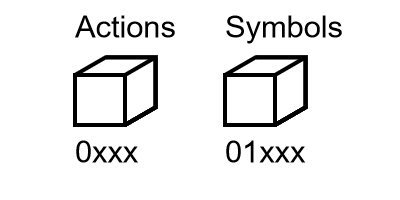
\includegraphics[width=\linewidth]{figures/figure1_cubes.png}

\caption{Action and symbol cube. Two cubes of course does not make a hypercube, it should be 8 cubes, but most of those are left for future additions to the full 8x8x8x8 hypercube of 4096 elements.}
\end{figure}




    The action cube consists of actions or sequences of actions which do something on the screen of a computer using discrete geometry.  They all use a set of global geometric variables which are manipulated during the drawing of a glyph in much the same way that registers are used in a traditional microprocessor.  These global variables include position of a cursor, angle of the cursor, a length scale, a factor for increasing or decreasing the length scale, a symmetry on which to carry out rotations, and a few other useful parameters.   





    Glyphs consist of sequences of actions.  They are expressed as strings in the form of base 8 addresses separated by commas, e.g.``0300,0341,0333,0341,''.  Some addresses in the action cube consist of glyphs, which in turn refernce other glyphs or actions.  Thus many levels of recursion are possible and used routinely.  This is a huge part of the power of this system over existing graphical systems like Adobe Illustrator.  Adding glyphs to the shape table and using those glyphs is not like just copying and pasting shapes in Illustrator.  It is in fact more like building up cell hierarchy in a electronic layout CAD program. 
    



    For each action in the action cube, be it a discrete JavaScript action or a glyph made of of other actions of glyphs, there is always a corresponding symbol glyph in the symbol cube, in the address space 01000-01777.  These symbols are \textit{
always} glyphs made up of a sequence of actions(rather than an action in JavaScript).  




    Both the action and symbol cube have a full 64 + 32 = 96 cells for the printable ASCII characters from space to tilde.  The standard printable ASCII characters go from space at 040 octal(0x20 hex, 32 decimal) to tilde at 0176(0x7E hex, 126 decimal), with 0177 being backspace which we leave as a``do nothing'' operation in the Geometron hypercube. The symbols at 01040 through 01176 are glyphs which constitute a font, stored in a file called font.txt.  The symbols in a font can use a full shape table of up to 64 specialized geometron action sequences, creating new fonts very quickly and with total flexibility even with no coding skills.  This is particularly useful for creating new fonts for specialized purposes such as programming easily into a robot or lithography tool. As with Chinese characters, the stroke order maters, each symbol is spelled with a specific order of actions, and the order matters.   


\begin{figure}
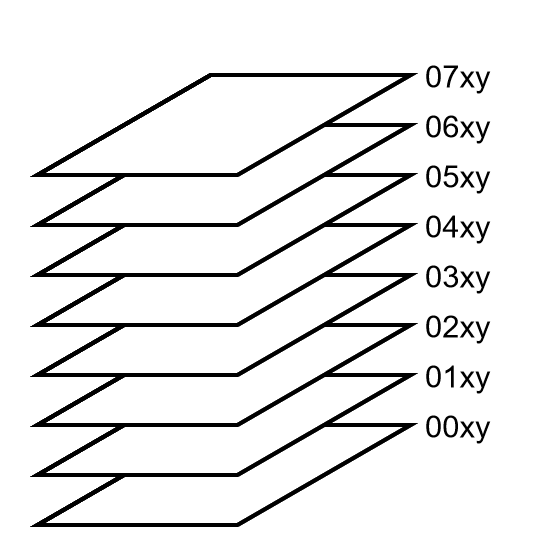
\includegraphics[width=\linewidth]{figures/fig2cubestack.png}
\caption{Tablet layers.}
\end{figure}

    The Geometron Action Cube is divided up into layers, called tablets, each of which is a 8x8 array, much like a chess board.  Those tablets are then broken up into rows of 8 actions, which we attempt to group in a rational way.   

\begin{figure}
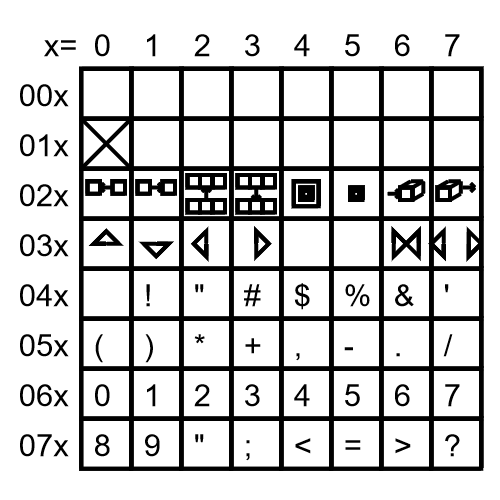
\includegraphics[width=\linewidth]{figures/figure3_bottomTablet.png}

\caption{Figure 3. Bottom Tablet.  This is split between the bottom part of the printable 7 bit ASCII code and various system actions which control things like cursor position while editing glyphs. }
\end{figure}

    The bottom tablet in address space from 0 to 077 consists of ``root magick'' actions from 06 through 037 and the first part of the ASCII from 040 to 077.  Root magick consists of actions which are not purely geometric in nature, which interact with the Geometron software.  Examples of these are ``move cursor forward'', ``move cursor back'', zoom and pan of the view of the glyph, moving through the shape table in the shape table editor etc.  As with all other parts of the Action Cube, each action has a symbol in the Symbol Cube.  The first six elements of the bottom tablet are left open for storage of HTML and creation scripts in more self-contained versions of the code(to be discussed elsewhere).  


\begin{figure}
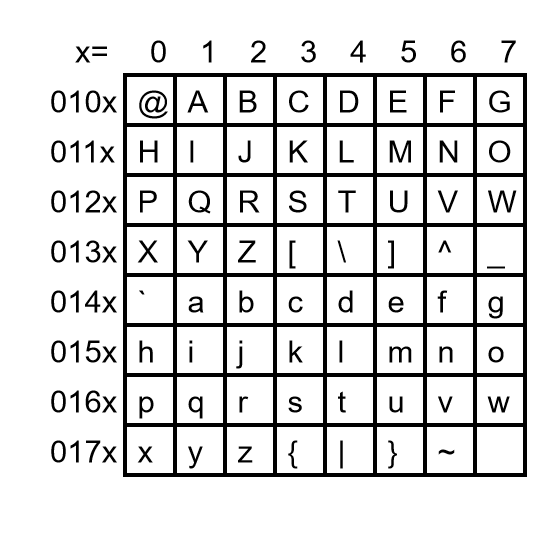
\includegraphics[width=\linewidth]{figures/figure4_asciitablet.png}
\caption{First tablet from bottom: top of 7 bit ASCII.  Backspace at 0177 is excluded and replaced by a ``do nothing'' action.  Hence range is from ``at'' symbol(0100) through tilde(0176), or 0x40-0x7E hexidecimal.}
\end{figure}

    The second tablet is the top part of the 7 bit ASCII code, from 0100(the @ symbol) to 0176(tilde ~).  These addresses are used for different things in different contexts. In the storage of the Hypercube, they each contain a single address, which creates a map from all the possible keys including shift keys on a standard keyboard, and this is used to make custom Geometron keyboards of all kinds, and makes it easy to edit those keyboards, making infinity of versions of the keyboard.  Depending on context, however, the ASCII actions can also add letters to the ``Word stack'', a global string variable which gets dumped out into printed words in various contexts.



\begin{figure}

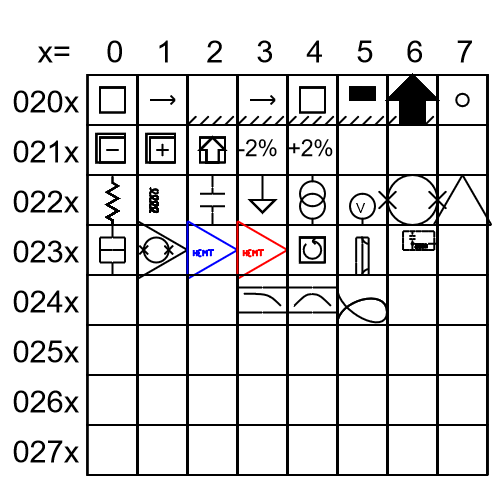
\includegraphics[width=\linewidth]{figures/figure5_shapetable.png}

\caption{Shape table.}
\end{figure}

    The third tablet is the shape table.   This begins with ``base shapes'' from 0200 through 0217 which are glyphs that are used so often that it makes sense to keep them mostly fixed.  This includes the ``cursor glyph'' which is at address 0207, and is how spelling of glyphs and the live cursor correlate with each other.  Also, the square is at 0200 which is used so more than pracicaly any other shape since it encapsulates the symbol glyphs.  The range from 0220 through 0247 are the standard ``shape table'' which most language instances use.  The work flows described later in this paper are based on these shape tables, and that is how languages like ``quantum gates'' or``superconducting circuits'' are encoded.  These tables are all of the format of newline delimited sets of glyphs with an address in the format ``0200:0362,0203,0334,0203,0334,0203,0334,0203,0334,0354,".  



\begin{figure}

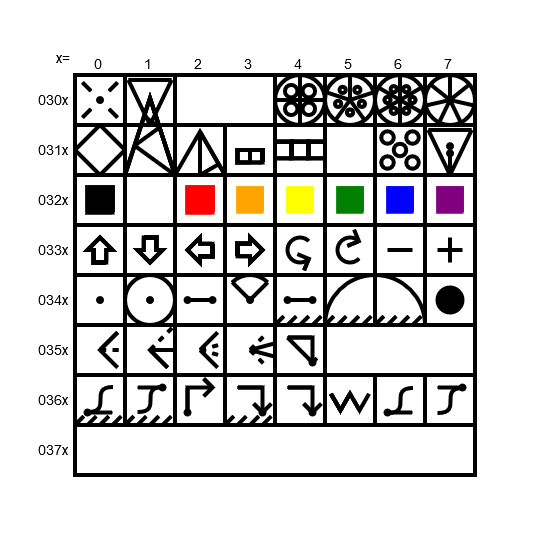
\includegraphics[width=\linewidth]{figures/figure6_actionTablet.png}

\caption{Action Tablet}
\end{figure}

    The fourth tablet, from 0300 through 0377 is the main Action Tablet, which are simple sets of JavaScript statements all accessed through one function called doTheThing() which takes integers as inputs and selects out various actions which either modify the global variables or take actions on SVG and canvas elements(both).  Note that since the ASCII code is a subset of the Geometron Hypercube, from address 040 through 0176 that all the JavaScript code can still be considered to be of the form where each cell in the action cube consists of an array of addresses, since a ASCII string can be encoded as addresses.  

    Addresses from 0400 through 0777 are left open in the current instance of Geometron presented here. Leaving this huge space in the addresses open leaves a large range of possible applications open using this geometric function.  Each of these tablets is by convention some different type of information and like 03xx they are generally some type of human readable code, such as HTML, CSS, JavaScript, python or JSON.  Another use of this section of the hypercube is to allow creation of totally new geometric action sets which apply to Hilbert space manipulations of the state of a quantum processor, as well as virtual reality 3d constructions, both of which will be dealt with in another white paper. 


\begin{figure}
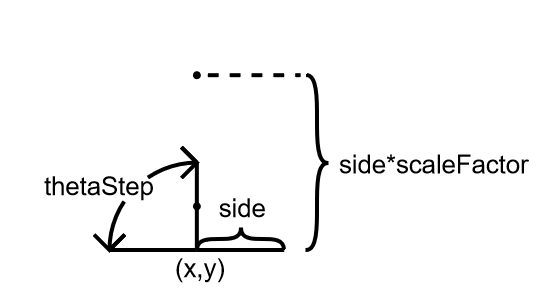
\includegraphics[width=\linewidth]{figures/figure7_globalCursor.png}
\caption{Global graphical cursor}
\end{figure}




    When actions are carried out, they manipulate global geometric variables, which are expressed by the state of a global graphical cursor.  The cursor is itself a glyph like any other, and is located at address 0207, in the base rows(0200-0217) of the shape tablet.  The symbol glyph 01207 is a small circle, which looks like the period in traditional Chinese writing.  The cursor has a base which is located at (x,y), a direction which shows the angle ``theta'', wings which show the step angle thetaStep, and a pair of dots which show the scale factor called scaleFactor.  




\begin{figure}
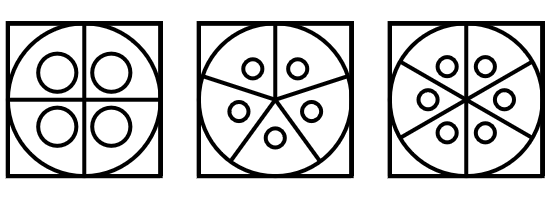
\includegraphics[width=\linewidth]{figures/figure8_symmetries.png}
\caption{Basic symmetry groups.  These glyphs correspond to setting the angle step to be 90 degrees($\frac{\pi}{2}$ radians), 72 degrees($\frac{\pi}{5}$ radians), or 60 degrees($\frac{\pi}{6}$ radians). Their addresses are 0304, 0305, and 0306. }
\end{figure}


    Angles of rotation are discrete and all start from some basic rotation groups, shown in Figure 8.  These are based on 4 fold, 5-fold, and 6-fold symmetry.  A further set of actions includes bisecting and trisecting angles as well as their opposite, which allow for symmetry groups of multiples of these basic numbers and their prime factors(3 and 2 can be made from doubling 60 degrees to 120 or 90 degrees to 180.)  Note that while classical compass and straightedge geometry is a guide in the construction of geometron, I have chosen to ignore it when the computer allows and it is convenient as in the case of trisecting arbitrary angles(not possible in classical construction).      

    A natural way to extend Geometron for some specific applications is to add other symmetry groups to the action row 030x, such as 7 or some other weird higher prime number.  Extending these types of operation to much larger numbers might be a path to implementing factorization of large integers in quantum geometron using Galois theory, which will be discussed in another white paper.


\begin{figure}

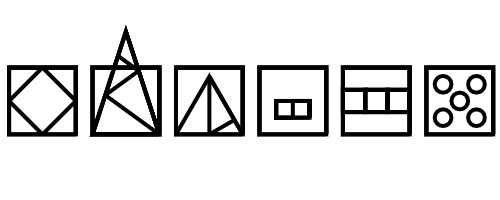
\includegraphics[width=\linewidth]{figures/figure9_scales.png}

\caption{Scale factors.  $\sqrt{2}$, $\phi = \frac{1 + \sqrt{5}}{2}$, $\sqrt{3}$,2, 3, and 5, which are at addresses 0310, 0311, 0312, 0313, 0314 and 0315.}
\end{figure}


    Scale factors are chosen to conveniently relate to the standard angles used in the symmetries and their close relatives.  They are on the row 031x in the Action Tablet, and are organized in order of size of the scaleFactor value.  For instance the square root of two allows us to easily make a 45 degree isosceles triangle by first setting stepAngle to 45 degrees by bisecting 90 degrees, then with scaleFactor equal to square root of two, one application of the``increase scale'' action at 0337 increases the side length by square root of two, making it the right length for the hypotenuse no matter what the current side value is.  Similarly, the square root of 3 allows for easy and rapid construction of 30/60/90 right triangles at any scale, and smooth navigation of hexagons and equilateral triangles, and the Golden Ratio provides the same for pentagons, pentagrams, Penrose Tiles etc.  


\begin{figure}

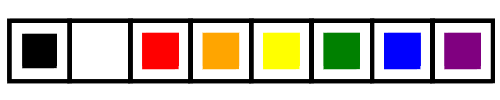
\includegraphics[width=\linewidth]{figures/figure10_layers.png}

\caption{Figure 10. Layers/colors.  These are at addresses 0320 through 0327.}
\end{figure}


    The action row 032x selects layers, which each have a space in a global style structure, and determine width and color of lines as well as fill color. In the web based Geometron presented here, this simply maps to style in a canvas or SVG element.  However, this can be easily adapted for other more literal layer concepts if we are constructing Geometron instances for things like nanofabrication and other literal physical implementations.  By default, the colors roughly follow the rainbow.




\begin{figure}

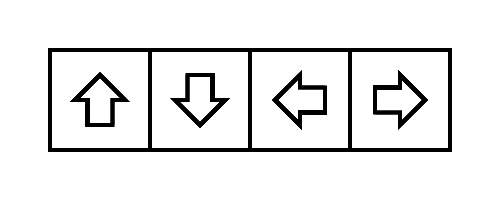
\includegraphics[width=\linewidth]{figures/figure11a_movements.png}
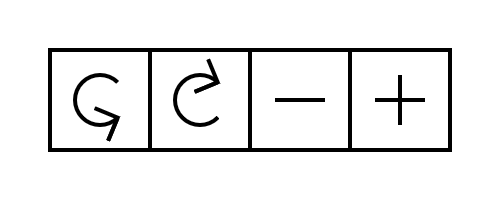
\includegraphics[width=\linewidth]{figures/figure11b_rotationscale.png}

\caption{Figure 11a,b. Basic movements: discrete step in (x,y) space, rotation, increase or decrease scale.}
\end{figure}


    The movement row of the Action Tablet is at 033x, and includes moving the position either forward or backward on the direction``theta'' and along the direction of either of the``wings'' of the cursor, in the direction``theta + thetaStep'' or ``theta - thetaStep".  The rotation actions represent either increasing or decreasing theta by thetaStep.  Plus and minus represent increasing or decreasing ``side'' by a multiplicative factor of scaleFactor.  


\begin{figure}

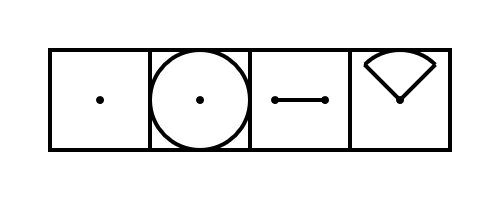
\includegraphics[width=\linewidth]{figures/figure12_basicDraw.png}

\caption{Figure 12. The most basic drawing actions: dot, circle, line segment, arc.}
\end{figure}

    There are numerous drawing actions which can be added to the Geometron Action Tablet, but the most basic self-contained geometric constructions are the dot, circle, arc and line segment.  These alone can be used to construct a very large class of diagrams, figures, symbols, etc.  

\begin{figure}

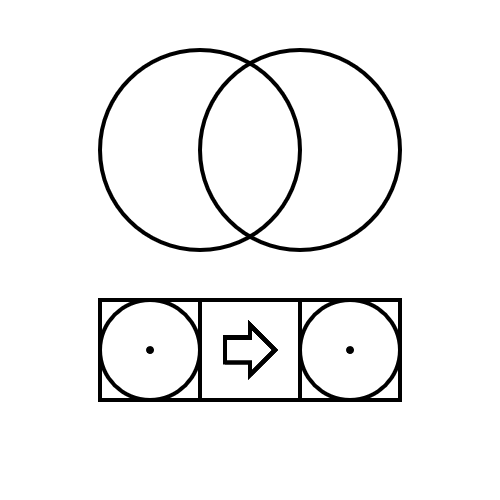
\includegraphics[width=\linewidth]{figures/figure13_vesicaPisces.png}

\caption{Figure 13. Vesica piscis, the ``hello, world'' of geometric language.}
\end{figure}


    The tradition in teaching and learning of computer programming languages of creating a program to print ``hello, World'' can be extended to geometric languages with the vesica piscis(from the Latin for fish bladder), which is two circles each centered on the other of same radius.  Technically the vesica piscis is the intersection area of the two circles, but since the double circle glyph is maximally simple we use that as the Hello, World of Geometron.



\begin{figure}

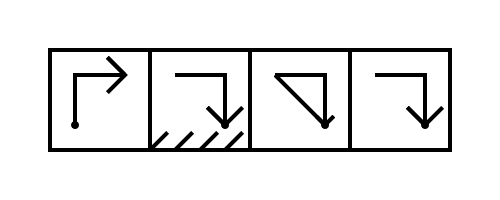
\includegraphics[width=\linewidth]{figures/figure14_paths.png}

\caption{Figure 14. Paths: a key element of all vector graphics systems.  The actions are: start path, close and fill, close and don't fill, and terminate without closing.  All three are very useful.  Several actions exist to connect these, including cubic Bezier paths, arcs and line segments.  A very common source of errors in geometron glyphs is paths that are not closed.  Always close your paths. }
\end{figure}


    Paths are a crucial component of all vector graphics, and Geometron is no exception.  We need to be able to start paths, then create shapes along them in the form of line segments, arcs and Bezier paths, then terminate them.  There are three ways to terminate a path: close and fill, close and don't fill, and don't close.  The glyphs for all of these are shown in Figure 14.  




    While there are some actions not discussed here, this concludes a basic survey of the most critical components of the Geometron Hypercube, which shows its basic structure and how it can be useful as a general purpose tool to construct new graphical languages.  I will not move on to show by example what this tool can do, focusing on its utility for the quantum information community.




\section{Examples}


    As with any language, there is no substitute for immersion and examples when learning Geometron.  Ideally the reader will be able to get guidance in recreating all these examples live on the Web, but for the purposes of a static white paper, this will just be a guided tour of example glyphs in Geometron which try to highlight how it can be of use for the quantum information community.



\begin{figure}

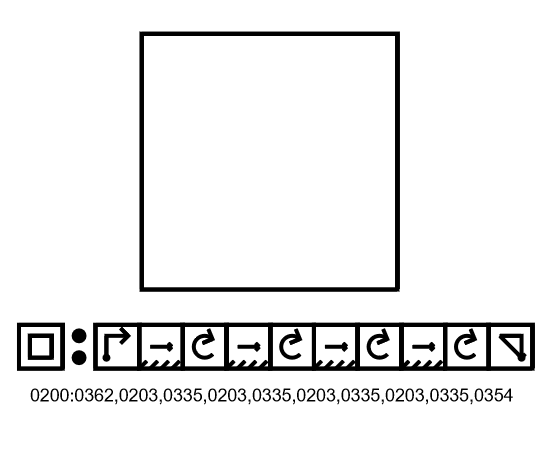
\includegraphics[width=\linewidth]{figures/figure15_square.png}

\caption{Figure 15. Square.  This figure is a closed path, so it has actions to both open the path and close it, separated by ``move along path'' actions, and rotations, which assume we are on a 90 degree symmetry.  A good exercise is to repeat this with 120 degree symmetry to get a triangle, with 72 degree to get a pentagon, and 60 degree symmetry to get a hexagon(these have more steps but are the same basic patttern.)}
\end{figure}




\begin{figure}

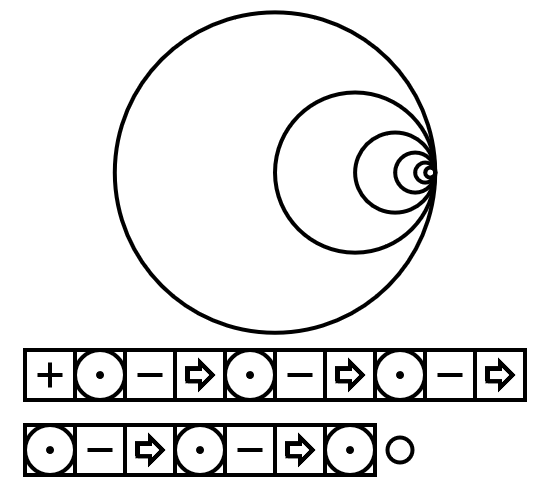
\includegraphics[width=\linewidth]{figures/figure16_circlesFractal.png}

\caption{Figure 16. Simple circles figure.  This figure, which is part of a Smith chart, is very simple to construct with just a few keystrokes in Geoemtron, and shows the power of this method for creating figures like this. }
\end{figure}




\begin{figure}

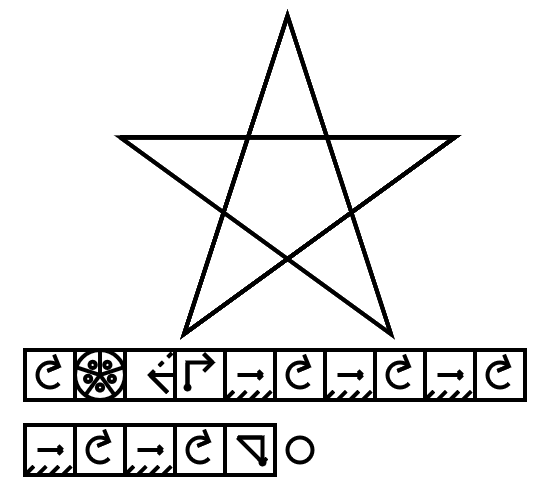
\includegraphics[width=\linewidth]{figures/figure17_star.png}

\caption{Figure 17. Five pointed star.  Creating a five pointed star is also just a few keystrokes, with the right symmetry selected, and with start/stop of closed paths, one can make either a filled or unfilled star in seconds with Geometron.}
\end{figure}





    The first three examples are just simple geometry: building a square, a fractal sequence of circles, and a five pointed star.  These are meant to give a feel for how rapidly simple geometry can be reliably reproduced with Geomtron, and for how it works.  




    The next set of examples build up a inductor for building circuit schematics.  While not explicitly quantum, no quantum circuit is without inductive elements, and they are by far the most frustrating element of vector graphics in the field to reproduce in high quality.  While one can also create a unit cell of the perfect inductor in software like Adobe Illustrator and just copy and paste it, the Geometron method has major advantages in how it scales to larger and more complex creations, and how it deals with complex custom circuits based on the inductor.   




    Once a unit cell is built, making any length of inductive elment is possibly by simply chaining together that unit cell action.  This means that just a few keystrokes can be used to create many different possible geometries of transformer for instance.  It also means that it is very easy with a couple of lines of code to create inductive circuits algorithmically. Once a compound glyph has been constructed such as the standard inductor, it can be joined with other glyphs in the quantum circuits shape table to make an RLC ciruit as shown in figure 22.  


\begin{figure}

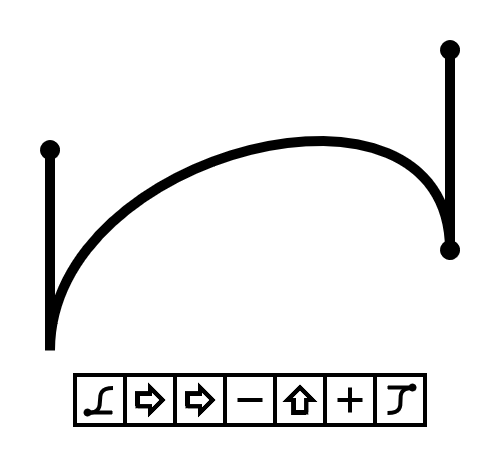
\includegraphics[width=\linewidth]{figures/figure18_coilBezier1.png}

\caption{Figure 18. Cubic Bezier path which starts the construction of a inductor.  Note that with discrete Geometron-based actions, this is a much simpler task than with continuous vector graphics editors.  With no access to existing electronic data, one can reconstruct this on another computer just from reading the printed symbol glyphs in the proper order.}
\end{figure}




\begin{figure}
    
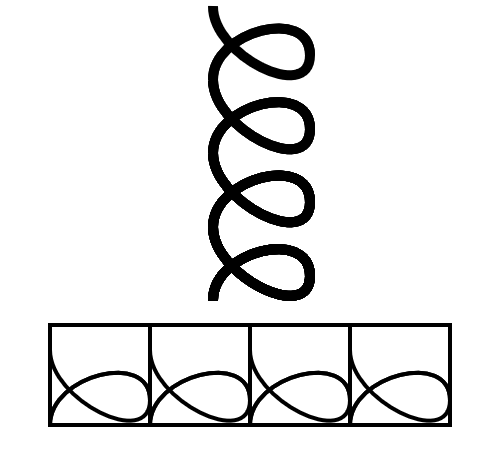
\includegraphics[width=\linewidth]{figures/figure19_inductor.png}

\caption{Figure 19. An inductor built up from individual loop glyphs.}
\end{figure}



\begin{figure}

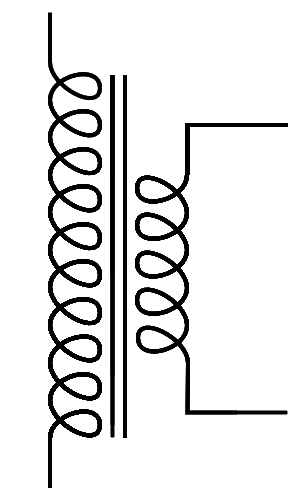
\includegraphics[width=\linewidth]{figures/figure20_transformer.png}

\caption{Figure 20. Transformer made from same sub-elemets as simple inductor.  Building circuits like this begins to show the labor-saving power of Geometron: this is just a few actions, but can now be encoded as a shape, so a single action can instance it, allowing the user to build up huge complex inductive circuits with very little effort or artistic skill. }
\end{figure}



\begin{figure}

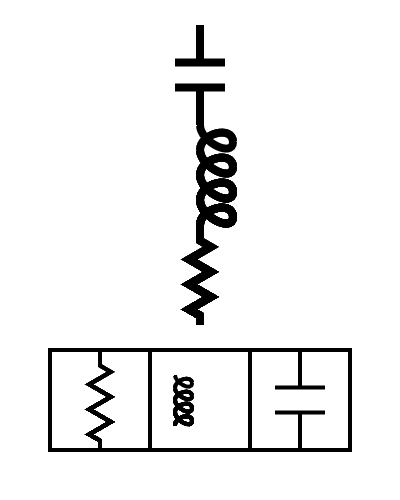
\includegraphics[width=\linewidth]{figures/figure21_rlc.png}

\caption{Figure 21. RLC resonator circuit.}
\end{figure}



\begin{figure}

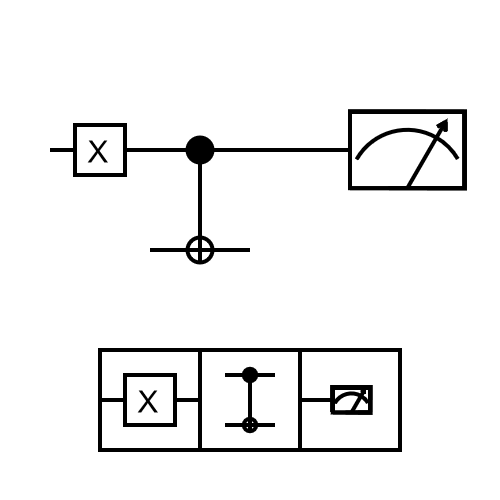
\includegraphics[width=\linewidth]{figures/figure22_gates.png}

\caption{Figure 22. Quantum gate symbol construction and glyph spelling.}
\end{figure}




    Construction of sequences of quantum gates is done by simply chaining gate drawing actions together into a glyph as shown in Figure 22. Gates are in turn made of of various sub-glyphs such as the generic box which contains the X, Y, Z, S and T gates, or the bottom part of a control-not.  This means that new gates can very easily be constructed and then deployed across the whole space of graphics in use.  Since these glyphs are very small amounts of simple numerical information in the form of the addresses of each action, they can easily be made into the output of a very simple quantum processor, leading to self-programming quantum computers with minimal effort.




\begin{figure}

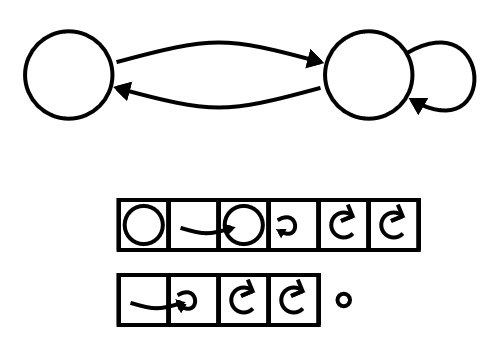
\includegraphics[width=\linewidth]{figures/figure23_graphtheory.png}

\caption{Figure 23. Graph theory constructions using a Geometron instance of arrows and circles.}
\end{figure}




   Graph theory has proven to be a very useful tool in quantum information science and technology, with applications in several branches.  Creating the diagrams of graph theory is also just a sequence of simple actions such as ``create node, make a path to the next node, create that node, make a self-loop'' etc.  In the form presented in this white paper, the output is simply the circles, arrows and lines in SVG or PNG format, which must then be annotated with symbols in another program.  The software presented in the next white paper however will show how with a decentralized graphical social networking system it is possible to add formatted math to these graphs and publish them on the Web very quickly. 



\begin{figure}

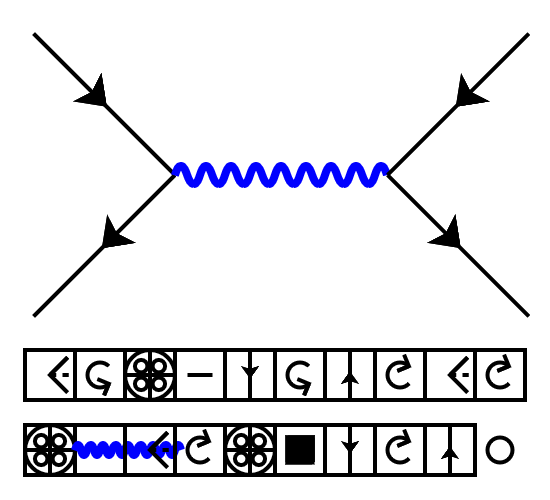
\includegraphics[width=\linewidth]{figures/figure24_feynman1.png}

\caption{Figure 24. Building a Feynman Diagram from individual sub-glyphs, with spelling shown below.}
\end{figure}




    Finally, no tour of graphical languages for quantum theory would be complete without a eample Feynman diagram.  The power of those simple cartoons to reduce the labor associated with calculating path integrals is a major motivating force for this work: it proves that the simple act of drawing a new type of cartoon can have a large impact in what workers in a computational field can achieve.  Figure 24 shows how a Feynman diagram is built up from constituent actions, which can be re-arranged to make other diagrams. 

\section{Structure of Code}


    All the code that makes up the Geoemtron system designed to run in the browser, using standard HTML, CSS and JavaScript.  The one exception to this is communicating with the filesystem which is all done with PHP, and that is part of a social media structure which will be documented in another white paper.  




    The main function of the Geometron Virtual Machine is called doTheThing(), and it is a JavaScript function which acts on an integer representing an address in the Geometron Hypercube discrete address space from 0 to 01777.  Depending on the address, this function does different things as described in section 2.  The core actions are all in the range from 0300 through 0377, and consist of either drawing shapes or altering the state of the global variables which change over the course of the drawing of a glyph.  




    Glyphs are drawn using a function called drawGlyph(), which acts on strings in the Geometron Bytecode Format.  The Geometron Bytecode Format consists of a sequence of octal numbers separated by commas in a string.  E.g. the glyph representing the ``hello world'' of geometry, the vesica pisces, is ``0341,0333,0341,''.  A trailing comma is optional.  Thus if we write drawGlyph("0341,0333,0341,") from the console when Geometron is running in the browser, the glyph will be split up into an array of strings each of which represents a number, then each number will get converted to int and sent to doTheThing() in order.  This will lead to drawing a circle one ``side'' in radius, moving by ``side'' in the x direction to the right, then drawing another circle of the same radius.   




    The commands which draw are designed to simultaneously control the canvas element and a global string variable called currentSVG, which will be used to create SVG images when the SAVE SVG button is pressed.  For example, the draw circle action in doTheThing(localcommand) is 


\begin{verbatim}
    if(localCommand == 0341){
        ctx.beginPath();
        ctx.arc(x, y, side, 0, 2 * Math.PI);
        ctx.closePath();
        ctx.stroke();
        currentSVG += "    &ltcircle cx=\"\";
        currentSVG += Math.round(x).toString();
        currentSVG += "\" cy = \"";
        currentSVG += Math.round(y).toString();
        currentSVG += "\" r = \"" + side.toString() + "\" stroke = \"" + currentStroke 
            + "\" stroke-width = \"" + (ctx.lineWidth).toString() + "\" ";
        currentSVG += "fill = \"none\" />\n";		
    }
\end{verbatim}


    As stated, this combines actions on a global canvas context variable called ctx and the SVG text, which will be both saved to a SVG file and exported to the textIO textarea element.   

    Code for a Geometron instance is edited on the server itself, using the Ace.js javascript library which allows for a code editor to be embedded in the browser.   A file called editor.php allows a user to edit separately all of the various components of a Geometron instance, which are divided up by type of code into JavaScript, HTML, CSS, PHP, Geometron Bytecode, and JSON.  

    Code is further divided by function, so for instance the JavaScript code has separate files for the initialization function init(), the function which draws the screen after each user interaction called redraw() and various types of actions in doTheThing.  A single file called index.php calls each of these little pieces of code each time a user's browser calls it, so that the most recent version of each section of code is used on that loading.  

    The main working screen of Geometron includes a large number of features which can be subtracted in some instances for specific applications.  The whole structure of the code is self-replicating, meaning that just one small PHP script needs to be copied to a web server, and that will fetch all the rest of the code from another existing Geometron server and set up the whole system locally.  

    The basic operation of Geometron consists of a user placing their cursor in a input in the upper left corner of the browser, then hitting keys which trigger a JavaScript event.  This event maps keys to actions, which can be anywhere in the Geometron Hypercube.  The value of these actions is itself stored in the hypercube, and can be changed on the fly as needed for specific applications.  Creating a new glyph in this way is very similar to creating a sequence of ASCII characters in a text document.  When one hits most keys, they add on action to where the glyph is, but arrow keys and backspace move the cursor through the glyph or delete an action.  As the cursor moves through a glyph, the user will see both the circle cursor move through the glyph spelling at the bottom of the screen and see the graphical cursor move its location and format through the sequence of the glyph.  This is very important, as it allows one to see the current state of the global variables along the sequence of actions before inserting an action in the middle of a glyph.  


\section{Workflow}

There are three levels of interaction a user can have with Geometron.  At the minimal level of interaction, one consumes graphical content as it is made availalbe, simply using the free Public Domain vector graphics that are made available for ones own work.  The next and most common level of interaction is learning how to make your own graphics, and using an existing Geometron instance to do that, creating custom graphics for whatever media you're working on.  The third level of involvement is to build up your own graphical languages, making custom tables of symbols for whatever your technical application or branding might require.  This is where the true power of Geometron will be unleashed: when people in the community start to build and share their own new graphical languages.  One might think of this as a sort of meta-Feynman diagram: a general system for diagramatically solving new types of problem in quantum theory(or indeed any field).  It is my hope that each of these work flows leads continuously into the next, with people using the graphics, learning a little of the language, then getting hooked on how much fun it is to make interesting diagrams quickly, start making their own for fun, and eventually incorporating this into their main graphical workflow, and finally when they're very comfortable in the language, building their own symbolic languages(which is the same commands you use to make any symbol.)

The graphical languages I focus on on www.quantumart.org are quantum circuits(circuits with Josephson juncitons), quantum logic gates(based on the introduction to Nielson and Chuang), Feynman diagrams, and simple knot theory for topological applications.  The static libraries just focus on the quantum circuits and the logic gates to keep the signal to noise ratio of the library high.  

    There are three main work flows I will discuss here.  The first is simply a free vector graphics library for the quantum information community, maintained at www.quantumart.org.  This is intended to be grown over time and to attempt to have as many commonly used symbols as possible, all explicitly in the Public Domain, with as many format choices as possible for very smooth use in existing graphics workflows.  The second is use of the specific graphical languages (geometron instances) for quantum information, which are also provided at www.quantumart.org.  These ``graphics factories'' can be used to rapidly create, publish, edit and share vector graphics using graphical languages specificlaly for QI.  This includes quantum logic gates, quantum circuits, Feynman diagrams, and graph theory diagrams. The third work flow is full instancing of the metalanguage, where the user creates their own graphical languages, both symbols and actions.  This is where the true power of this system will be unleashed, especially when paired with the technical micro-blogging software documented elsewhere.  

There are two ways to parse the work flow of the Geometron system.  We can consider the path taken by a new user, which is what is sketched in the above paragraph.  In this flow, a new user starts out seeing this as just a free graphics library, then moves up to making their own graphics, and finally to building their own graphics languages.  The other way to consider the work flow is to trace the path of the information as it would flow for an expert user.  In this path, a Geometron instance is created by cloning all the code using the script replicator.php onto a new directory on a web server with PHP istalled.  

Full Workflow:
\begin{enumerate}

\item Read this paper, learn goals of Geometron, decide to learn it.
\item Browse existing graphics libraries, download whatever vector graphics or bitmap images are of use to you for your own library.
\item Navigate your Web browser to an existing Geometron instance, try some basic operations with your keyboard to get a feel for how it works, move the cursor around, delete and edit glyphs, draw circles and lines, and some shapes
\item Make or have made your own custom Geometron keyboard for a further commitment to deplying it
\item Explore the system to make sure you can make the kinds of figures you need for your applications, learn to make and export and use PNG's and SVG's
\item Install your own instance of Geometron on your web servers or a local host inside your firewall, generally a Raspberry Pi
\item Rework the look and feel of the front page of your instance for the branding of your group/company/institution, working in collaboration with your front end Web developer team 
\item Construct your own shape libraries for the specific applications of your lab and your research and your technology and branding.  Share as much as you feel comfortable with, hopefully enlarging the graphical commons shared by the whole community.  
\item Create and share your own media feeds of SVG and png files with the rest of the world, sharing links to either your original graphics feed or a mirror of it if you're working behind a firewall.
\item Document your modifications to the code, spread the ideas to other quantum information groups, and teach them to replicate this entire workflow.


\end{enumerate}

First read this paper, focusing especially on the figures, and noting any errors or corrections to send to the author or further notes you want to add in your own documentation later.

The graphics library can be found at www.quantumart.org/library.  Peruse it at your leisure, share it widely use it as needed.  

To start with movements, load the browser to the page www.quantumart.org/sandbox, and the cursor should automatically be placed in the correct input for actions to happen so that all you need to do is hit keys.  Start with the keys a,s, d, and f(all lowercase) as wel as g, h, j and k.  These should move the cursor around, and give you a chance to see how that works.  Use the backspace key to delete an action from the glyph.  Use the left and right arrow keys to navigate the cursor through the action sequence of your glyph.  When the movement makes some sense, add the basic drawing actions z,x,c and v which are point, circle, line segment and arc.  

After these basic motions make sense, keep plyaing with them to try making some basic shapes and cartoons, but this will remain limited until you get used to it, and it's a good time to move on to the symmetries.  The three you mostly wan to play with are 90 degrees which is the back tic mark under the tilde in the far left of the top row of a standard ASDF keyboard, the 1 and the 2 keys, which are 72 degrees and 60 degrees respectively.  Also, 3 is bisect angle and 4 is double, 5 is trisect and 6 is triple angle.

Try differnt scale by going along the row from the angle commands to 7,8,9,0,- and = keys, which are all scaleFactor values.  Try different scale values and then zoom in and out with j and k to see how they work.  

make a Bezier

make a closed path, filled and unfilled

make text with 01xxx, with 0365

choose layers, use them

edit style JSON

export a png, save it to your computer

svae a svg, link to it, save it to your computer

publish a svg link, share it so others can edit on server and publish edits and share them

Build your own space on quantumart.org/yournamehere

Build your own server, hire me, build a pi locally, build graphics, share and publish on web using a mirror, customize the language, build a physical node for the network in a conference room with a custom keyboard and a projector on a big screen 

Customize your code for your brand and your research, publish it all, share your artwork as art 





Full workflow:

Read this paper(or skim it and look at the pictures) 
download free graphics for use in your documents from graphics library
try out basic movements, drawing actions, make circles, lines, and gates and circuits
make your own graphics on existing instance shared with you, publish them and use them as needed, learn to read the feeds of other users to also use their graphics productions
create new instance:
replicator.php
navigate to glyph editor, test:
index.php
go to tree, create a new branch on it:
tree.php
go to that branch and start editing it:
index.php?path=mynewpath/
edit the shape table:
shapetableeditor.php?path=mynewpath/
shapes.txt
pastebin.com 
actions, then symbols
index.php?path=mynewpath/
(PUBLISH)
svg/svg[datecode].svg $\rightarrow$ web, adobe creative suite, microsoft office suite, inkscape
(PNG PUBLISH)
save as: filename.png $\rightarrow$ powerpoint, word, latex, web
web links$\rightarrow$ svgfeed.php $\rightarrow$ index.php?path=mynewpath/&url=mynewpath/svg/svg[datecode].svg
share and spread to other users, teaching them how to create an instance, use it, modify it and spread it themselves so that the entire system self replicates and evolves based on user needs.  

deep dive into code, improve it
get web developers to work over the CSS of your instance to brand it and make it fit with the rest of your web presence, build replicator with instructions for how to fork on your page. 
tell other people who will go back to step 1.

replication is covered in the next white paper.
applying the concepts of geometron to quantum information processing is covered in the third white paper, quantum modeling in HTML.

Note that as this system propagates through the quantum information community, the flow of code will form a branching tree, with the earliest adopters of the system being the largest and deepest branches.  No special code skills are required for a researcher, group, institution or even lone hobbyist to have this role, just determination and artistic skill.  A motivated individual can have a large impact on the overall structure of the quantum information field by diving deeply into this system, building a large feed of graphics, and spreading those graphics enthusiastically to the rest of the community.  From a business and marketing standpoint, building an instance which people rely on  and which is branded with your company and biased toward the technology you're working on can have a huge global impact on your reach in the field without spending any money other than the time of everyone involved to learn the system.  





    Graphical documentation of quantum computing languages, simplifying the construction of programs as well as the sharing of them between various types of researcher or expert.




    Running on a local machine, Connecting with Jupyter notebooks and LaTex


Hire me to set up a local node of Network


\section{Future Work and Implications}

Try to imagine learning about quantum two level systems without the Bloch sphere, or basic gates without the graphical represntation of control not or quantum electrodynamics without Feynman diagrams.  These graphical tools are some of the most powerful we have at our disposal(including computers and lab equipment even) as quantum information scientists.  Imagine if the bar to build a new graphical language like this were lowered to where a graduate student could easily make a new one on their smart phone while waiting for the bus.  We have no idea just how much computational power will be unleashed by creating a free open graphical network for this kind of information, but the only way to find out is to build it.  


The work presented in this paper is simply a factory for graphics.  The next of the three white papers that present this work will deal with building a social network based on sharing information created with Geometron.  It is worth noting here that the World Wide Web was originially built by Tim Bernars Lee at CERN specifically to help physicists communicate with one another and to organize their research information.  I believe that it is a rational next step for the Web to build another such extension.  This next white paper will describe the Geomtron Network, which is a self-replicating system that allows for totally free rapid sharing of graphics and integration of math-formatted text with them.  It is integrated into a slide sharing system which can replace PowerPoint for rapid online sharing of graphics, and a paper authoring system which integrates with $\LaTeX$, and a system for making vector graphics from standard function plots we use frequently.  The key idea of this system is that the current most powerful form of communication of technical ideas is simple text fields superposed on top of simple graphics, and that the faster we can make and share these with the minimum possible friction, the more powerful our communication will be.  This whole system is also predecated on the idea that the future of information technology is self replication and evolution, that is the user runs simple code that replicates the whole code base to a server, where they can easily modify the code as they go along, then when they spread it to the next user, their new, modified code base is passed along, so there is no one centralized code base, but a rhizomnal network of flowing code through the network. 

The third of the white papers that makes up the sequence of Geometron for quantum information will discuss how Geometron can be used for creating sequences of discrete geometric actions in Hilbert space as well as in three dimensions just as it does in two dimensions in the system discussed here.  The thesis of this paper is that it should be possible to create Geometron instances for 3d virtual reality modeling of problems which are amenable ot quantum speedup in the browser, build another geomtron instance for the space spanned by the qubits in the quantum processor, then by building direct maps between these spaces to create a user interface for people solving these problems which truly leverages the power of Hilbert space geometry, without relying on models based on classical computer science.   I will describe a system for controlling and programming a quantum processor whereby a group of users simultaneously interact with the processor in real time using a multiplayer virtual reality interface, programming the machine using yet another geometron instance which describes qubit control pulses using discrete geometry.  Finally, by showing that the output of the quantum processor can also be geometron glyphs, I will show that this is a path to the self-programming quantum computer.



point to the other two main white papers: 
    Self Replicating Graphical Social Network for QI and 
    Quantum Visualization and Control in HTML

    microblogging for real time technical graphical communication




    Building geometric languages to program quantum computers without the numerical/English based intermediary.




    Decentralized art feed network, I will help you replicate the code on your server, then adapt it for your specific applications, and train your people to use it, build custom keyboards, link to other nodes on Quantum AR





Creating direct connections between the web browser and geometry of Hilbert space, to cut out the ``middle man'' between a quantum user and quantum circuit.  Real time quantum controls.    


    Create a language for protein structure using a custom GVM, another GVM for a many qubit hilbert space, then building a browser based UI for constructing purely geometric quantum algorithms which map problem space to hilbert space.  


    GVM for Galois groups, geometrizing the problems of factorization so that people can develop new algorithms for factoring using GVM.



\end{document}

